
\begin{figure}[h!]
    \centering
    \caption{Estimates of the effect of the minimum wage on rents, baseline sample
             including leads and lags}
    \label{fig:dynamic_baseline}

    \begin{subfigure}{.65\textwidth}
        \caption{Leads and lags of the workplace MW}
        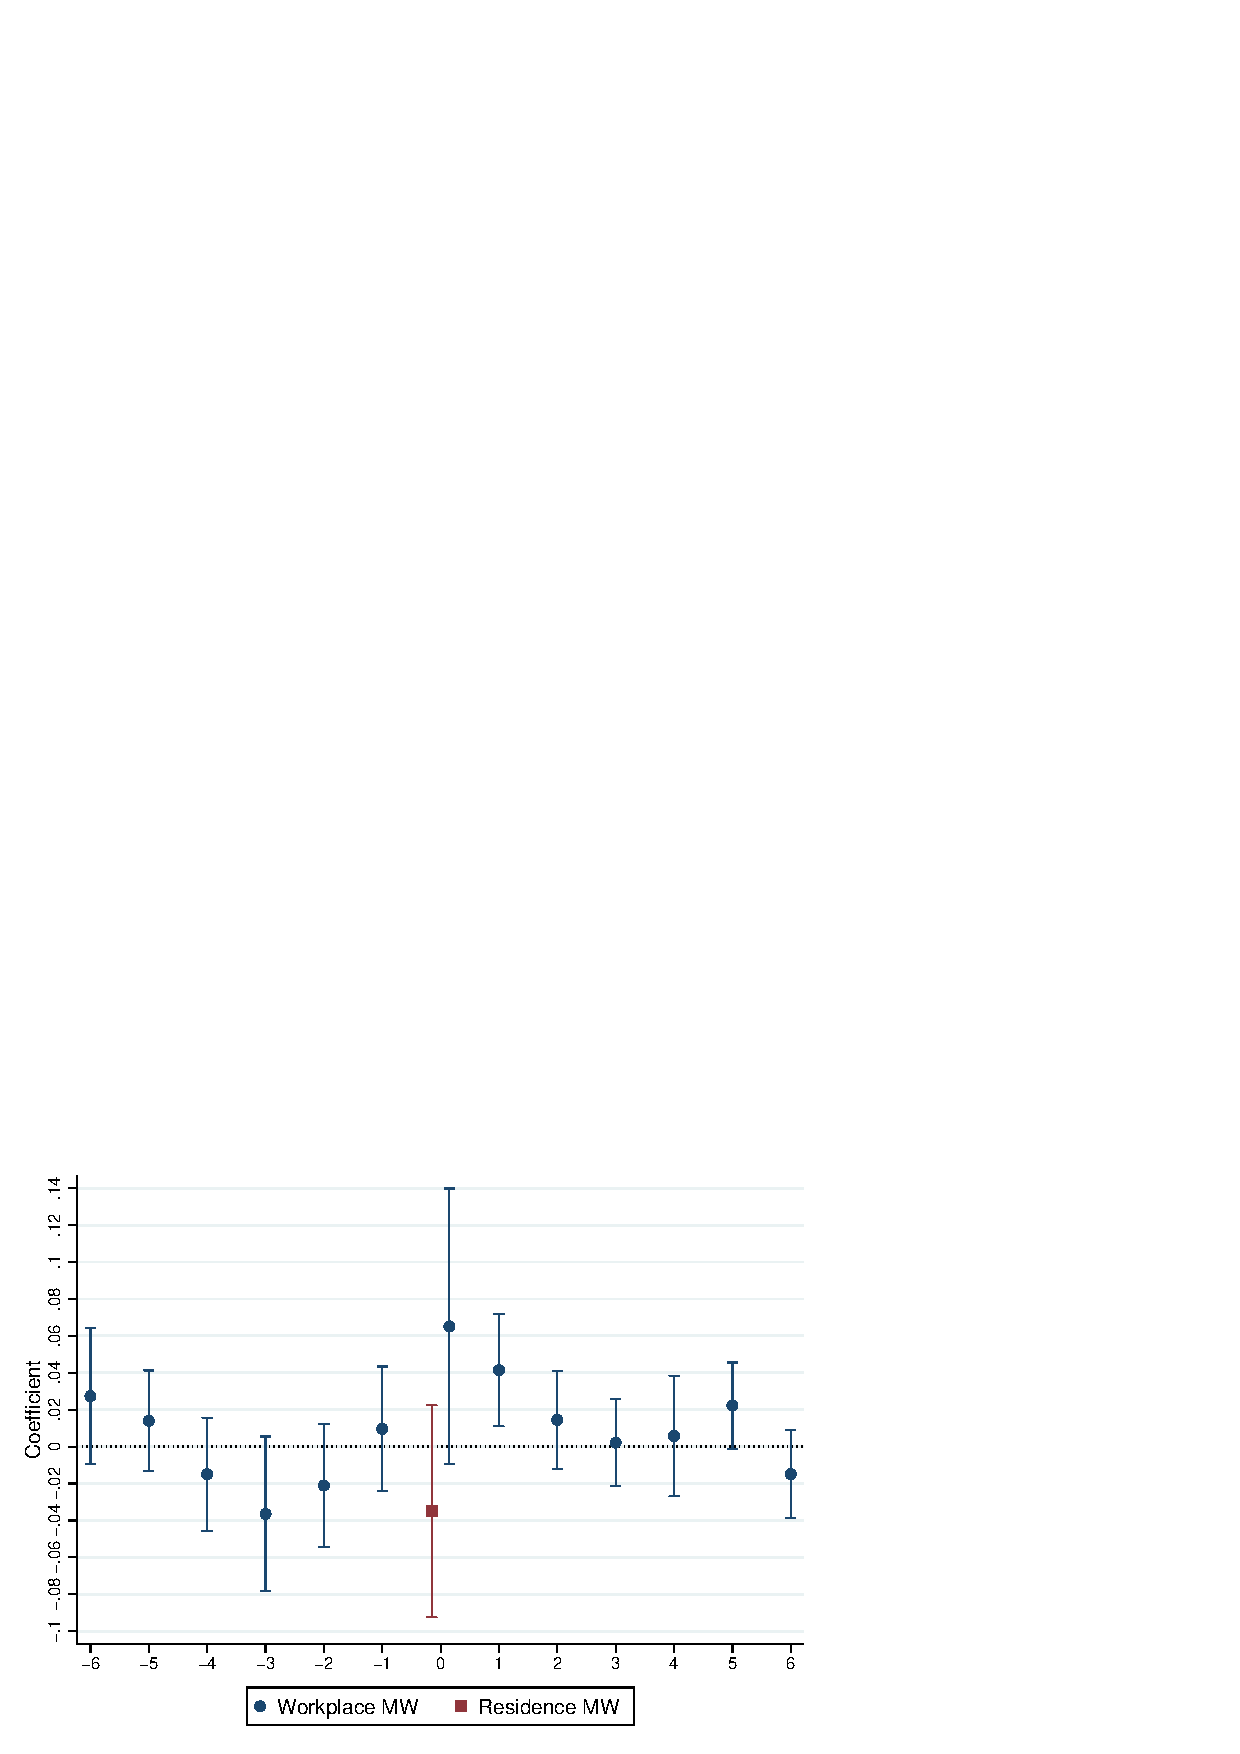
\includegraphics[width = 1\textwidth]
            {fd_baseline/output/fd_both_mw_wkp_only_dynamic}
    \end{subfigure}\\
    \begin{subfigure}{.65\textwidth}
        \caption{Leads and lags of the residence MW}
        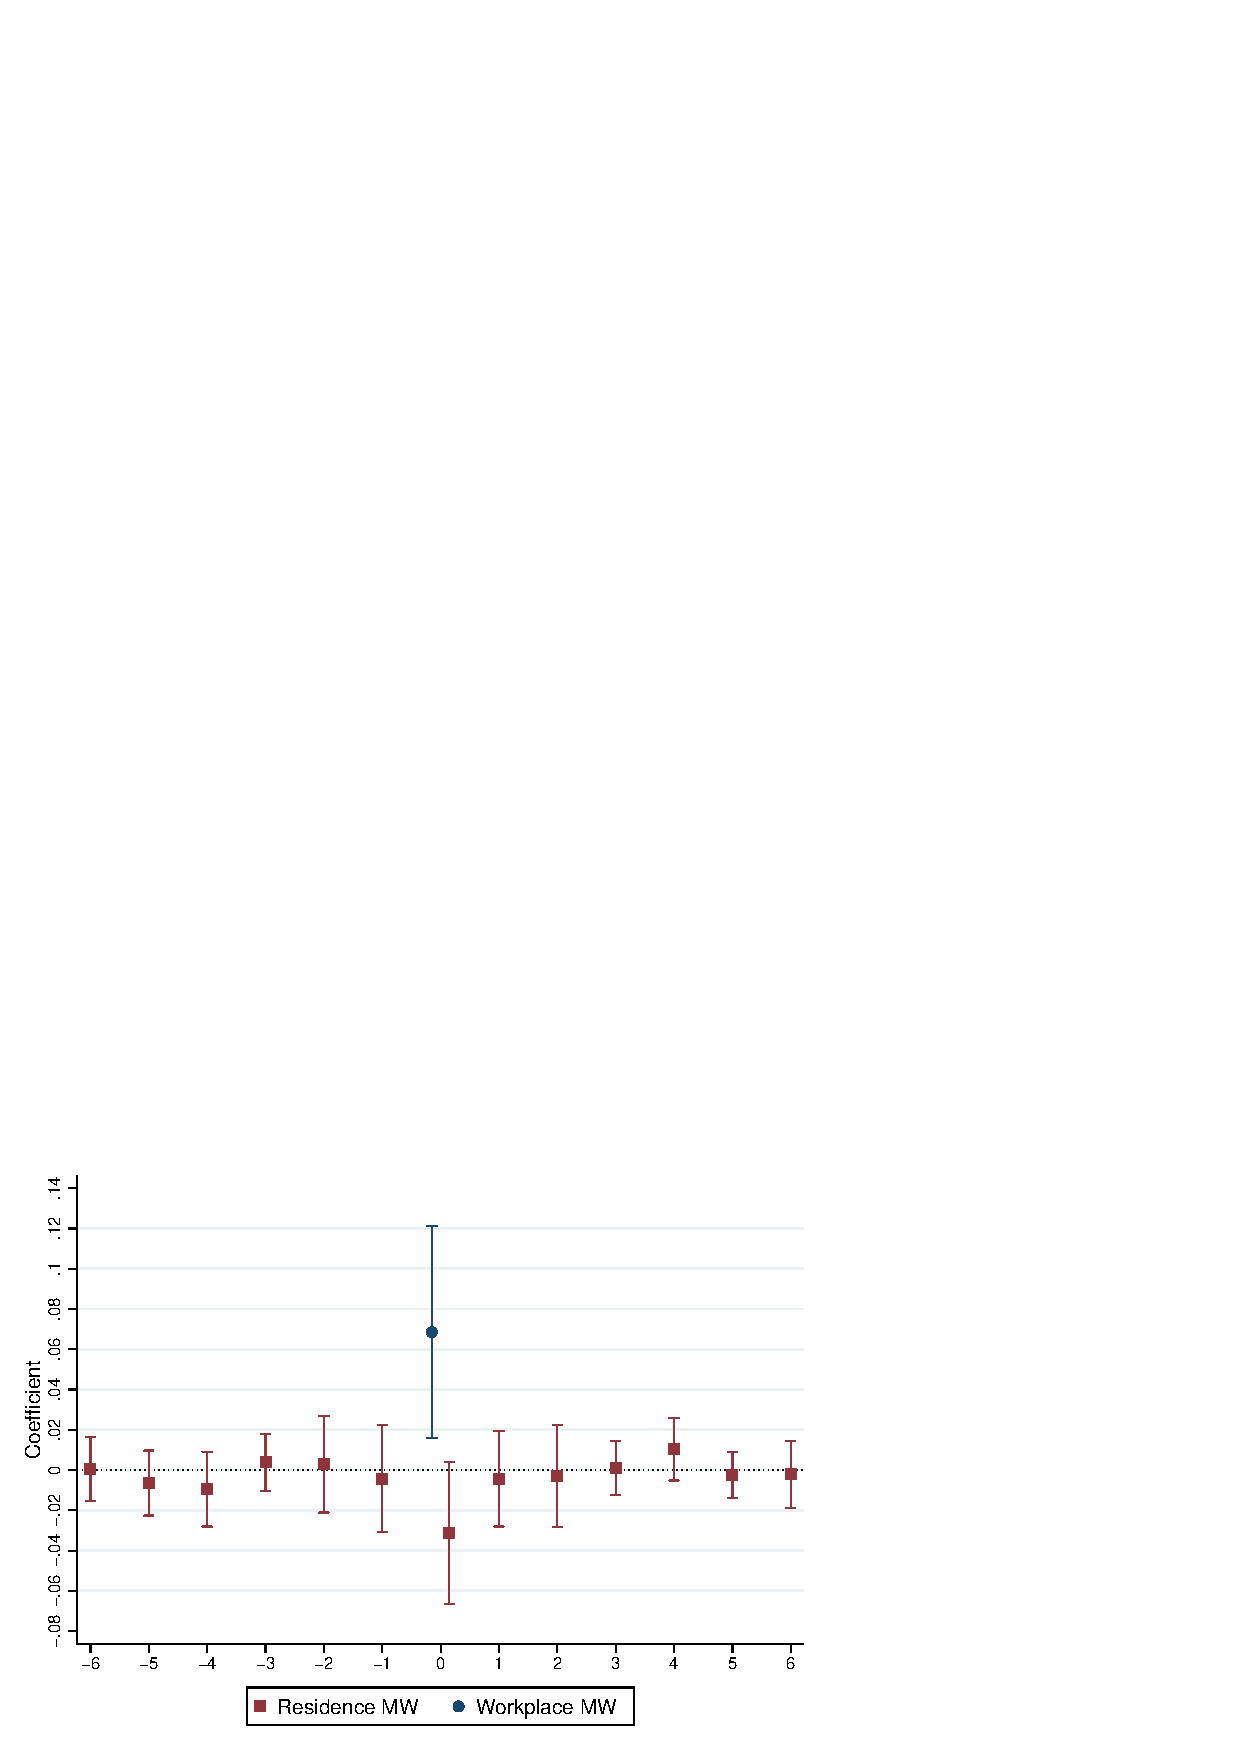
\includegraphics[width = 1\textwidth]
            {fd_baseline/output/fd_both_mw_res_only_dynamic}
    \end{subfigure}

    \begin{minipage}{.95\textwidth} \footnotesize
        \vspace{3mm}
        Notes:
        Data are from the baseline estimation sample described in Section 
        \ref{sec:data_final_panel}.
        All panels plot coefficients from regressions of the log of rents per
        square foot on the residence and workplace MW measures, varying the 
        number of leads and lags of each MW variable included.
        Panel (a) includes six leads and lags of the workplace MW measure.
        Panel (b) includes six leads and lags of the residence MW measure.
        All regressions are estimated in first differences and include 
        time-period fixed effects and economic controls that vary at the 
        county by month and county by quarter levels.
        The measure of rents per square foot correspond to the Single Family, 
        Condominium and Cooperative houses from Zillow described in Section
        \ref{sec:data_rents}.
        The residence MW is defined as the log statutory MW in the same ZIP code.
        The workplace MW is defined as the log statutory MW where the average 
        resident of the ZIP code works, constructed using LODES 
        origin-destination data described in Section \ref{sec:data_mw_measures}.
        Economic controls from the QCEW (Section \ref{sec:data_other}) include the
        change of the following variables: the log of the average wage, the log
        of employment, and the log of the establishment count for the sectors ``Information,''
        ``Financial activities,'' and ``Professional and business services.''
        95\% pointwise confidence intervals are obtained from standard errors 
        clustered at the state level.
    \end{minipage}
\end{figure}
